\section{Why Ants are so Small}

\begin{wrapfigure}{rt}{.3\textwidth}
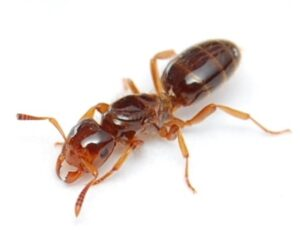
\includegraphics[width=.3\textwidth]{QueenAnt-300x248.jpg}
\end{wrapfigure}

\begin{quotex}
I enjoy nature shows. The world of insects is fascinating with its odd looking creatures, subtle beauty, and especially unbearable cruelty. They forged an evolutionary path distinct from the one that led to humans.
\end{quotex}

\begin{quotex}
And Solomon was David's heir. He said: ``O ye people! We have been taught the speech of birds and on us has been bestowed a little of all things: this is indeed Grace Manifest'' And before Solomon were marshaled his hosts, of Jinns and men and birds, and they were all kept in order and ranks. At length, when they came to a valley of ants, one of the ants said: ``O ye ants get into your habitations, lest Solomon and his hosts crush you under foot without knowing it.'' 
\flright{\textit{Surah} 27}
\end{quotex}

Once upon the time, three kingdoms developed: the jinn, the insects, and the vertebrates. They each inhabited their own worlds, with blurry boundaries between them. Hence, their respective worlds often collide, creating tensions. The jinns are the most ancient beings, followed by the insects and then vertebrates. The story of the jinns will have to wait until tomorrow since this is a story of the ants.

The world of the insects is largely unknown to humans, as they have their own hierarchies, food chains, and customs. However, the insects and vertebrates are often forced to interact with each other. This is not always bad because the ants are special creatures and can teach us many truths.

The ants and the bees sit at the peak of the insects and humans are the most evolved of the vertebrates. The insects developed along matriarchal lines, since in most insect species, the female is larger than the male. We all know that the female praying mantis devours her mate after coitus. This reaches full development in the ants. The productive part of the ant colony consists of females. The colony is protected by a race of Amazons that act as soldiers. The colony is ruled by the matriarch, called the queen. She retains, as a sort of anti-harem, some male ants, called drones, who are permitted to mate with her at a time she determines.

\paragraph{The Human Race}


Humans developed along a different line. Unlike ants, the males are larger. There is also an equal balance between the number of males and females. That is because the original human was an androgyne who split in two: male and female. Even when split apart through time and space, they remain entangled beings, not two, but one. Their spiritual task is to find each other and reach the unity of being. In some people, that attraction is quite strong.

\paragraph{Lust}


That attraction changes, at the physical level, into lust. Lust wants physical unity but not spiritual unity, carnal knowledge but not knowledge of the heavens. The patriarchy arose to control and channel such strong desires. Nevertheless, since vertebrates evolved from invertebrates, there is still a primordial memory of the matriarchy.

If human colonies were modeled like ants, then some females would garner the interest and attention of the males, so that many females would be neglected; clearly that defeats the real task of recognizing one's entangled other.

Some women are so beautiful to gaze upon, to remind men of the joys of Heaven. They adorn themselves with perfume, pretty shoes, nice dresses, and jewelry. The best among them are intelligent, articulate, and even spiritual. In an ant world, they would be queens, and men would gather around them like large groups of drones. You can see how disruptive that would be to human society.

\paragraph{The Jealousy of the Ants}


When the ants learned of the coming of humans, they had to make a choice about how to live, survive, and thrive in a world of large mammals. There were intense debates among the ants. Some wanted to modify themselves, through selective breeding, to become large also. This led to years of unsuccessful and dangerous experiments.

Finally, one of the princess ants rebelled and flew off to start a new colony of small sized ants. Since she was the most beautiful of all the ants, she was able to attract the best and strongest drones to go with as her mates.

\paragraph{The Wisdom of the Ants}


As the new smaller ants began to thrive, the older queen ants got jealous. They formed an alliances to attack the princess, now a powerful and beloved queen. But her soldiers were strong and well-disciplined and were able to defeat the larger ants, like the way David defeated Goliath.

These are the ants that spoke to Solomon.


\flrightit{Posted on 2021-07-02 by Cologero}

\begin{center}* * *\end{center}

\begin{footnotesize}
\begin{sffamily}
\texttt{Paulo Adolpho on 2021-07-08 at 02:02 said:}

Cologero, ants are the ideal communist society. There is a theory that says, that they are descendants of a species that degenerated and became that mechanized thing, that only thinks about work all day. Are robotic beings, depersonalized. If you take 20 workers, they are identical, if you take 20 soldiers, they are identical, the only differents, are the king and queen, just like the communist dictator, it is different from their mass subordinates. This is the path that humanity is taking, the path of massification, depersonalization, where work is the law and the state/leader is god

\hfill

\texttt{Cologero on 2021-07-08 at 23:02 said:}

Interesting take on it, Paulo, so your point is that the path of the ants is the superior biological choice. Either humanity begins to act like ants, or they will disappear from the earth.

\hfill

\texttt{Sylvan Savant on 2021-07-13 at 22:56 said:}

The greatest error of communism is its denial of human nature, not love and worship of the state. Because this ideology doesn't recognize human nature, it holds that the reformation of the external environment would also prompt the change in the inner state of the human organism. In other words, communists want to legislate grace as a matter of political fiat, which is a very convincing proposition if you reject the ontological given, i.e. the subject matter of metaphysics. Communist society is perfectly logical when you consider it as an empty set, i.e. a state of society in which there can be no human beings. In order to bring about this state of society, it is necessary to dehumanize people by abolishing the primary qualia that determine them to be such, whether it be religion, social hierarchy, race and gender.

\hfill

\texttt{Max on 2021-07-17 at 17:18 said:}

As the most advanced of the insects, the reproductive strategy of the beehive -- and I imagine the ants as well -- resembles that of humans. Not on the level of the individual insect, which behaves more like a single cell in its function, but regarding the hive as an organism in its own right. The hive will split at an opportune time, after which half will venture out to build a new hive, while the other half stays. In other words, it reproduces perhaps one offspring per year, at a very heavy investment. Likewise for sexual reproduction, the virgin queen flies out to meet up with a male from another hive, so that in effect two hives mate with one another. Another interesting tidbit is that the type of bee produced is not determined by genetics, similarly to how each human cell contains the same genetic code, which can then be expressed very differently depending on the function the cell in question is meant to serve in the body.

The organism of the beehive consequently does not know natural death, since it can regenerate its cells indefinitely. Each morning a few bees go out to scout for a good source of nectar, whereafter it returns to tell the directions of where sustenance can be found. Now, like the bees, we should get up every morning looking for the nectar of immortality. For these reasons, the Bee serves as a symbol for the immortality of the soul, and honey the food of heaven.

\hfill

\texttt{Max on 2021-07-21 at 07:45 said:}

``Go to the ant, thou sluggard; consider her ways, and be wise:

Which having no guide, overseer, or ruler,

Provideth her meat in the summer, and gathereth her food in the harvest.

How long wilt thou sleep, O sluggard? when wilt thou arise out of thy sleep?'' -Proverbs 6:6-9

Animals and fables is a favorite genre. The medievals, or ancient Israelites for that matter, understood animals in a different way than today. Solomon says that it is a ``grace manifest'', which is why it is so enjoyable to read their old accounts. I just resumed the Romance of the Rose, and the following passage is noteworthy for a comparable distinction as in the Surah abve, namely insect, man and angel:

``Ants and other small vermin could annoy men intensely if they knew their powers. It is true that their own natures are responsible for this ignorance, but, as for rational creatures, whether mortal men or divine angels, all of whom ought to praise God, if such a creature is so foolish as not to know himself, this failing is the result of wickedness, which dulls and fuddles his senses, for he is perfectly capable of being guided by reason and using his own free will, and nothing can excuse him from doing so.'' -The Romance of the Rose

The larger context in which this discussion occurs is that animals possess many powers, some even greater than man, although they lack the self-knowledge and will to direct those freely. For example, having understanding, ``... the elephant, who blows and trumpets though his nose and uses it to feed himself night and morning, as a man does his hand, would never bear a castle high up on his back.'' Instead of being like an animal, the author says that ``he alone loves wisely who knows himself thoroughly,'' meaning that true love is conditional. Continuing our study, we also learn that it is reasonable for fish to follow the stream, even though they make exceptions once in a while, thus demonstrating that recent events are not novel, despite what sophists might try to assert:

``And when the rivers overflow their banks, the fish that follow the streams, as is right and reasonable, since these are their homes, roam like lord and masters over the fields and meadows and vineyards to find food. (... ) The fish are also guests in nearby low-lying towns, which they find wretched and mean. They install themselves everywhere; no barn or cellar escapes, nor any place, however valuable and costly. They enter temples and churches to rob the gods of their service, and drive the household gods and their images from the darkened rooms.'' -The Romance of the Rose

Animals often do their best to distract us, dirupting religious services, but not because of reason. The fish have evidently visited these same wretched towns many times previously, and are just having a quick look-around, perhaps grabbing some scraps left in the pantry, before returning to their habitations. There is nothing new under the sun, as Solomon says. Priestly types, even today, still like to scare people with climatic events as punishments for their sins. Sometimes I wonder whether beings like the jinn or even angels look at humans and their antics like we do the ants.


\hfill

\end{sffamily}
\end{footnotesize}

